%----------------------------------------------------------------------------------------
%	TITLE PAGE
%----------------------------------------------------------------------------------------

\newcommand*{\titleGP}{\begingroup % Create the command for including the title page in the document
\centering % Center all text
\vspace*{\baselineskip} % White space at the top of the page

\rule{\textwidth}{1.6pt}\vspace*{-\baselineskip}\vspace*{2pt} % Thick horizontal line
\rule{\textwidth}{0.4pt}\\[\baselineskip] % Thin horizontal line

{\LARGE \textbf{国际教育-小学系列} \\[0.3\baselineskip] \textbf{中文版}}\\[0.2\baselineskip] % Title

\rule{\textwidth}{0.4pt}\vspace*{-\baselineskip}\vspace{3.2pt} % Thin horizontal line
\rule{\textwidth}{1.6pt}\\[\baselineskip] % Thick horizontal line

\scshape % Small caps
\href{https://fieldworkeducation.com/about}{Fieldwork-Education}\\[\baselineskip] % Tagline(s) or further description
\href{https://fieldworkeducation.com/curriculums/primary-years}{IPC}\par % Location and year

\vspace*{4\baselineskip} % Whitespace between location/year and editors

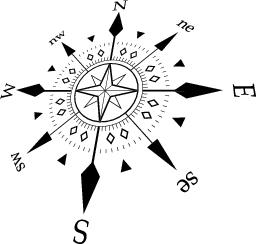
\includegraphics[width=10cm]{compass}


\vfill % Whitespace between editor names and publisher logo

{\itshape2398419426@buaa.edu.cn\par} % Editor list
{\itshape HaotianMichael \par} % Editor affiliation
\vspace*{0.5\baselineskip}
{\scshape 2018} \\ 
{\scshape Powered by \LaTeX \\[0.3\baselineskip]} % Year published

\endgroup}
